\chapter{Aspects techniques}

	\section{Représentation d'un livre}

		\subsection{Représentation des noeuds}
			Il y a quatre types de noeuds représentées par des classes (Voir figure \ref{fig:BookNode}): \textbf{BookNodeWithChoices}, \textbf{BookNodeWithRandomChoices}, \textbf{BookNodeCombat} et \textbf{BookNodeTerminal}.

			\begin{figure}[H]
				\centering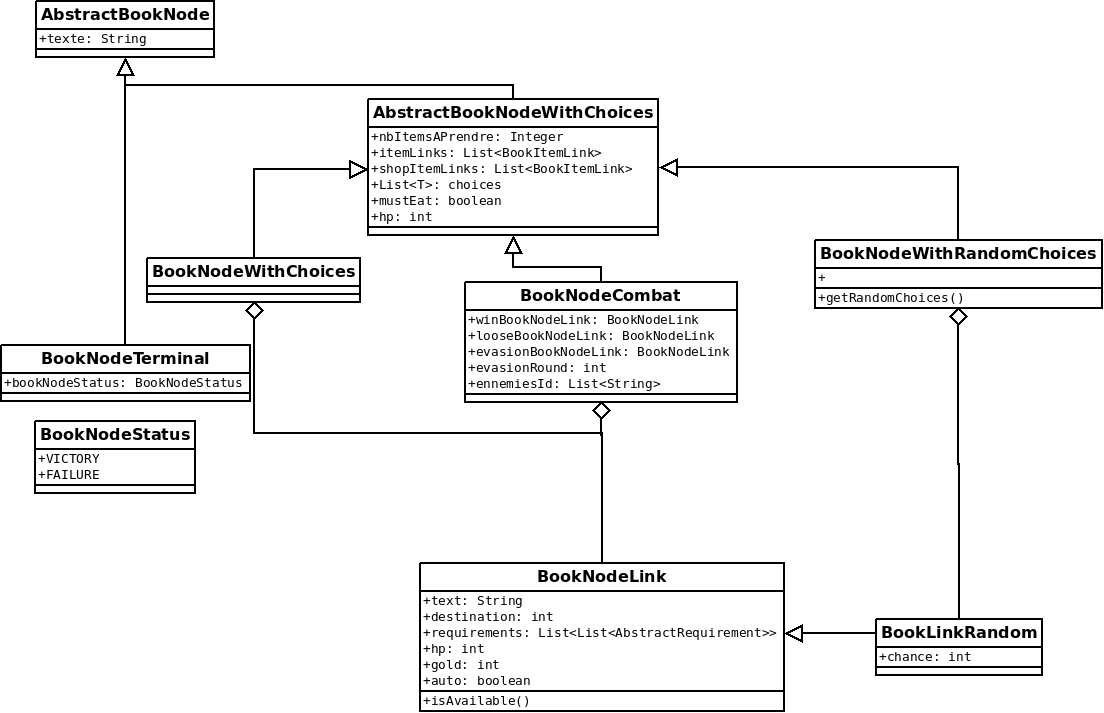
\includegraphics[width=0.70\textwidth]{img/BookNode.png}
				\caption{BookNode}
				\label{fig:BookNode}
			\end{figure}

			Tous extends direct ou indirectement de \textbf{AbstractBookNode}. Cette dernière contient juste un texte correspondant aux paragraphes de chaque noeuds.

			Pour le \textbf{BookNodeTerminal}, il prend en compte, en plus du texte de \textbf{AbstractBookNode}, une énumération (\textbf{BookNodeStatus}) qui ne prend en compte que \textbf{FAILURE} ou \textbf{VICTORY}.

			Pour l'ensemble des autres noeuds, on retrouve une liste de choix et une perte/gain de vie. Pour cette raison, elles extends toutes d'une même classe \textbf{AbstractBookNodeWithChoice} permettant ainsi de définir des variables tel que la liste des items disponible sur ce noeud, le nombre d'item maximum qu'on peut en prendre, la liste des items qu'il est possible d'acheter, le nombre de vie perdue / gagnée sur ce noeud, mais aussi, et surtout, la liste de choix disponible. Ce dernier est défini par une List<T> car cela peut être un \textbf{BookNodeLink} ou un \textbf{BookNodeLinkRandom}. Nous avons fait le choix d'utiliser un généric sur la classe \textbf{AbstractBookNodeWithChoice} afin de définir la classe utilisé pour la liste de choix. De cette manière, on empêche un noeud random (\textbf{BookNodeWithRandomChoices}) de contenir des choix "normaux" (\textbf{BookNodeLink}). Il ne peut contenir que des \textbf{BookNodeLinkRandom}, c'est à dire des choix avec une probabilité d'être choisi.

			Pour le BookNodeCombat, le choix a été fait d'ajouter 3 BookNodeLink afin de représenter les différentes issues du combat : victoire, evasion, defaite. Une liste contenant les ID des ennemis que l'on doit combattre y est également renseignée. De plus, ce noeud peut également posséder les même attributs que AbstractBookNodeWithChoices. Raison pour lesquels il en hérite. Nous avons donc redéfini les méthodes spécifiques aux choix, c'est à dire celle pour récupérer les choix, celle pour les supprimer et celle pour les mettre à jour. La liste de la classe mère n'est plus utilisable. Il s'agit d'une grosse erreur de notre part. En effet, cette classe demande un traitement spécial à presque tous les endroits où l'on peut gérer des noeuds. Il aurait plutot fallu ajouter les choix dans la liste parente et avoir un moyen de faire une distinction afin de savoir lequel est celui de victoire, de défaite ou d'évasion. On aurait pas eu à redéfinir autant de fois des comportements particuliers pour ce noeud avec des instanceof. Par manque de temps et au vu des changements importants que cela nécessitait, pour faire cela proprement nous n'avons pas pus changer cela.

			Pour le \textbf{BookNodeWithRandomChoices}, une méthode a été ajoutée, afin de sélectionner un choix de manière aléatoire en fonction de la probabilité de chaque lien. Pour cela, on ajoute d'abord tous les liens disponibles dans une liste nommée listNodeLinkDisponible. C'est à dire, les liens où le joueur peut avoir accès en fonction des prérequis demandés. Si aucun lien n'est disponible, cela retourne null. Dans le cas contraire, on choisit un nombre aléatoire en fonction de la somme totale des probabilités des liens valides ( Voir listing \ref{getRandomChoices}).\\
			En fonction de ce nombre, la probabilité de chaque lien valide est enlevée du nombre tiré jusqu'à ce qu'il soit égal ou inférieur à zéro. Le choix sélectionné est alors retourné (c'est la destination).

			\begin{lstlisting}[gobble=12, language=java, label=getRandomChoices, caption=getRandomChoice()]
				int nbrChoice = 0;
				Random random = new Random();
				int nbrRandomChoice = random.nextInt(somme);
				for (int i = 0 ; i < listNodeLinkDisponible.size() ; i++){
					if(!this.getChoices().get(i).isAvailable(state)){
						continue;
					}
					nbrRandomChoice -= this.getChoices().get(i).getChance();
					if(nbrRandomChoice < 0){
						nbrChoice = i;
						break;
					}
				}
				return this.getChoices().get(nbrChoice) ;
			\end{lstlisting}


		\subsection{Représentation des liens}
			Les noeuds sont liés par des liens. Ces liens sont soit défini par la classe \textbf{BookNodeLink} ou \textbf{BookNodeLinkRandom}. Pour éviter les redondances, cette dernière extends de \textbf{BookNodeLink}. Elles prennent donc toutes les deux un texte, une destination (défini par le numéro du noeud) et enfin, une liste de prérequis.  Pour la destination, nous avons d'abord mis un \textbf{AbstractBookNode}, mais beaucoup de manipulations étaient nécesssaires lorsqu'un changement était apporté au noeud. Nous avons alors choisi de changer et de mettre le numéro du noeud suivant. Pour plus d'information sur la gestion actuelle des noeuds, voir \nameref{book} à la page \pageref{book}.
			Pour le \textbf{BookNodeLinkRandom}, la classe à besoin d'une variable pour gérer la probabilité, afin de définir la chance d'aller vers ce noeud. Cette probabilité est ensuite totalisé sur tous les noeuds disponibles, comme vu précédement \nameref{getRandomChoices}.\\
			La classe \textbf{BookNodeLink} est composé d'une méthode, nommé isAvailable() permettant de savoir si le personnage principal rempli les conditions, défini par List<List<AbstractRequirement>>, pour aller vers ce lien. Pour savoir si le player peu aller vers ce lien, un appel de la fonction isSatisfied()\ref{isSatisfied}, vu un peu plus loin, sera utilisé afin de savoir si le personnage rempli la condition demandée (item et/ou skill et/ou monnaie). Si le player satisfait tous les prérequis demandés, cela retourne true. False dans le cas contraire.

			\begin{lstlisting}[gobble=12, language=java, caption=exemple de isAvailable(), label=isAvailable]
				for(List<AbstractRequirement> groupRequirement : requirements) {
					boolean satisfied = true;
					for(AbstractRequirement r : groupRequirement) {
							if(!r.isSatisfied(state)) {
								satisfied = false;
								break;
							}
						}

					if(satisfied)
						return true;
				}
			\end{lstlisting}

		\subsection{Prérequis pour un choix}
			Les prérequis des liens sont défini par une classe mère AbstractRequirement puis une classe par type de prérequis (requirements). Il y a la classe \textbf{RequirementItem}, \textbf{RequirementMoney} ainsi que \textbf{RequirementSkill}. Tous extends de AbstractRequirement afin de pouvoir redéfinir la méthode isSatisfied(), prenant en paramètre l'état du jeu (BookState). Tous prennent un ID en compte, permettant de retrouver l'item / skill / monnaie demandé. Seul le RequirementMoney possède une méthode qui diffère, c'est la quantité de money requis.\\
			Pour savoir si un item / skill est présent dans l'inventaire du personnage principal, une for est utilisée afin de regarder les items / skill possédés. Si l'ID de l'item / skill n'est pas possédé, le personnage principal ne peut satisfaire les prérequis. Pour l'argent grâce à l'ID de la monnaie, cela permet de savoir si le player en possède suffisament. Actuellement, une seule monnaie est disponible, se nommant "gold". En effet, nous n'avons pas eu le temps de le gérer dans les fichiers et dans le jeu.

			\begin{lstlisting}[gobble=12, language=java, caption=exemple de isSatisfied(), label=isSatisfied]
			public boolean isSatisfied(BookState state) {
				for (String i : state.getMainCharacter().getItems()){
					if(i.equals(itemId)) {
						return true;
					}
				}

				return false;
			}
			\end{lstlisting}


		\subsection{Représentation des personnages, items}

			Nous allons maintenant parler des personnages et des items du livre. Bien qu'il n'y ai pas grand chose à expliquer sur eux, car il s'agit de classes possédant beaucoup de getter et setter, nous souhaitons détailler certains choix faits.

			Commençons par les personnages. Ceux ci sont définits par la classe \textbf{BookCharacter} dans le package magic\_book.core.game. Cette classe possède presque uniquement des getter et setter bien qu'elle possède également quelques méthodes utilitaires.

			\begin{figure}[H]
				\centering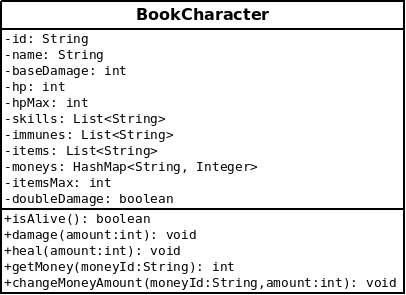
\includegraphics[width=0.45\textwidth, keepaspectratio]{img/book_character.png}
				\caption{UML sur la gestion des personnages}
			\end{figure}

			Concernant les listes de String (skills, immunes, items), il s'agit d'une liste contenant les id. Pour "immunes", il s'agit des ID des skills contre lesquels le personnage est immunisé. Cela permet aux items et aux compétences de n'être référencés qu'à un seul et même endroit, c'est à dire, dans la classe \textbf{Book}. Pour la monnaie, on a choisi d'utiliser une HashMap<String, Integer> afin de pouvoir gérer différents types de monnaie et leur montant dans une même histoire. Malheureusement, notre format de livre, et donc notre application, ne permet pour le moment pas de gérer pleinement cette fonctionnalité.

			Passons maintenant aux items. Ceux-ci possèdent une classe mère BookItem dans le package magic\_book.core.item.

			\begin{figure}[H]
				\centering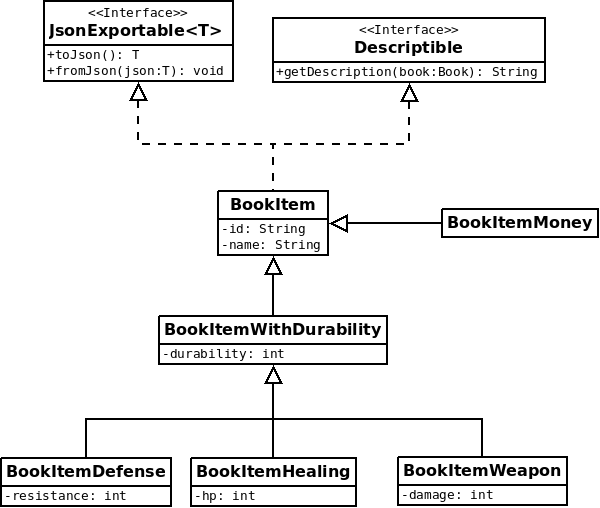
\includegraphics[width=0.66\textwidth, keepaspectratio]{img/book_item.png}
				\caption{UML sur la gestion des items}
			\end{figure}

			Avant de détailler notre choix, nous allons expliquer brièvement les deux interfaces que l'on observe. L'une se nomme \textbf{Descriptible} et permet à l'item de se décrire sous forme de String. Bien que la méthode \textit{String toString()} soit déjà prévu à cet effet, celle ci ne permet pas de prendre en argument un livre (classe \textbf{Book}). Bien entendu, c'est logique mais certains objets ont besoin du livre pour se décrire, par exemple, pour retrouver un item / personnage à partir de son id. La seconde interface, \textbf{JsonExportable} sera expliqué plus en détails dans \nameref{subsec:lecture_ecriture_fichier} à la page \pageref{subsec:lecture_ecriture_fichier}. Pour rester bref, disons qu'elle permet, la lecture et l'écriture du fichier en JSON.

			Dès lors, l'héritage prend son sens et permet une spécialisation d'un item de deux façons. La première, qui est la plus logique, permet l'ajout d'attributs spécfiques à notre classe fille. Par exemple, il serait étrange d'avoir un attribut pour savoir combien de dégat un item de type monnaie inflige. Deuxièmement, cette spécialisation intervient dans la redéfinition, par les classes filles, des méthodes des deux interfaces. En effet, chaque classe fille apporte ses propres attributs à chacune des différentes méthodes comme on peut le voir sur le listing ci-dessous. On nottera l'appel à la méthode définit dans la classe mère par le mot clé \textit{super.nomMethode(arguments)}.

			\begin{lstlisting}[gobble=12, language=Java, caption=Exemple de spécialisation des items]
			@Override
			public String getDescription(Book book) {
				StringBuffer buffer = new StringBuffer();

				buffer.append(super.getDescription(book));

				buffer.append("Dégats : ");
				buffer.append(damage);
				buffer.append("\n");

				return buffer.toString();
			}

			@Override
			public ItemJson toJson() {
				ItemJson itemJson = super.toJson();

				itemJson.setDamage(damage);
				itemJson.setItemType(ItemType.WEAPON);

				return itemJson;
			}
			\end{lstlisting}

		\subsection{La classe Book}\label{book}

			Cette classe est la plus importante de tout le projet. En effet, c'est elle qui met en lien tout les différents éléments qu'on a pu évoquer avant. C'est en effet ce que l'on peut observer sur la figure suivante.

			\begin{figure}[H]
				\centering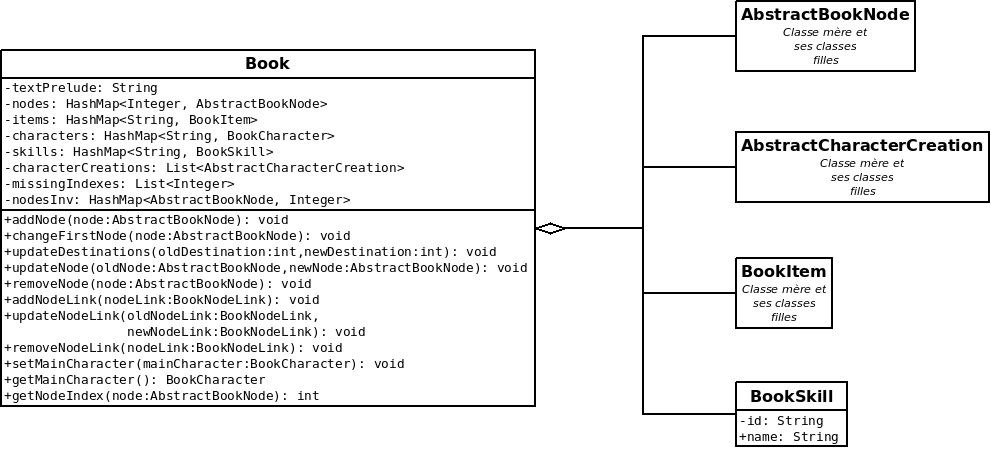
\includegraphics[width=0.8\textwidth, keepaspectratio]{img/book.png}
				\caption{UML sur la classe Book}
			\end{figure}

			Par soucis de place, les getters et setter n'ont pas été renseignés. Il en va de même pour le détails des différentes classes (\textbf{AbstractBookNode}, \textbf{BookItem}, ...). Enfin, les observateur sont volontairement omis car ils seront détaillés un peu plus tard (dans \nameref{subsec:pattern_observer} à la page \pageref{subsec:pattern_observer}).

			Tout d'abord, commençons par expliquer comment sont sauvegardés les noeuds et les liens dans la HashMap "nodes".

			Cette HashMap possède un int comme clé, qui correspond au numéro du paragraphe. Lorsque l'on ajoute un noeud au livre, on doit d'abord lui trouver un numéro. Nous avons décidé de plusieurs règles. Les paragraphes commencent à partir du numéro 1. Le numéro 1 représente \textbf{toujours} le premier paragraphe du livre. De ce fait, si l'on ajoute un noeud, il devra avoir pour numéro le 2.

			\begin{figure}[H]
				\begin{center}
					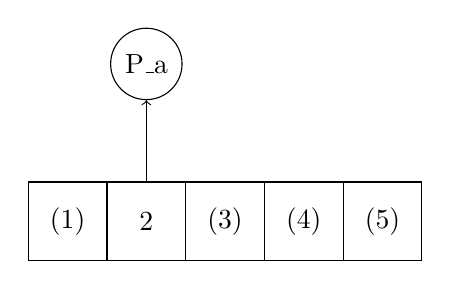
\begin{tikzpicture}
						\node[draw=black, text=black, shape=rectangle, minimum width=1cm, minimum height=1cm] (m_1) at (0,0) (1, 1) {(1)};
						\node[draw=black, text=black, shape=rectangle, minimum width=1cm, minimum height=1cm] (m_2) at (1,0) {2};
						\node[draw=black, text=black, shape=rectangle, minimum width=1cm, minimum height=1cm] (m_3) at (2,0) {(3)};
						\node[draw=black, text=black, shape=rectangle, minimum width=1cm, minimum height=1cm] (m_4) at (3,0) {(4)};
						\node[draw=black, text=black, shape=rectangle, minimum width=1cm, minimum height=1cm] (m_5) at (4,0) {(5)};

						\node[draw=black, text=black, shape=circle, minimum size=0.5cm] (p_a) at (1,2) {P\_a};

						\draw[->] (m_2.north) -- (p_a.south);
					\end{tikzpicture}
				\end{center}
				\caption{Ajout du paragraphe A}
			\end{figure}

			Les autres numéros sont représentés mais mis entre parenthèse car ils n'existent pas dans la Map. Ils sont uniquement là pour nous aider à bien visualiser ce dont on parle. Si nous décidons maintenant d'ajouter un second paragraphe alors celui-ci sera à la position 3.

			\begin{figure}[H]
				\begin{center}
					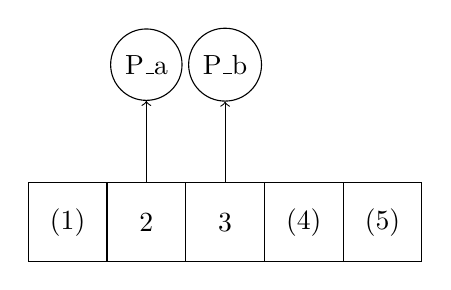
\begin{tikzpicture}
						\node[draw=black, text=black, shape=rectangle, minimum width=1cm, minimum height=1cm] (m_1) at (0,0) (1, 1) {(1)};
						\node[draw=black, text=black, shape=rectangle, minimum width=1cm, minimum height=1cm] (m_2) at (1,0) {2};
						\node[draw=black, text=black, shape=rectangle, minimum width=1cm, minimum height=1cm] (m_3) at (2,0) {3};
						\node[draw=black, text=black, shape=rectangle, minimum width=1cm, minimum height=1cm] (m_4) at (3,0) {(4)};
						\node[draw=black, text=black, shape=rectangle, minimum width=1cm, minimum height=1cm] (m_5) at (4,0) {(5)};

						\node[draw=black, text=black, shape=circle, minimum size=0.5cm] (p_a) at (1,2) {P\_a};
						\node[draw=black, text=black, shape=circle, minimum size=0.5cm] (p_b) at (2,2) {P\_b};

						\draw[->] (m_2.north) -- (p_a.south);
						\draw[->] (m_3.north) -- (p_b.south);
					\end{tikzpicture}
				\end{center}
				\caption{Ajout du paragraphe B}
			\end{figure}

			Maintenant, supposons que nous souhaitons que notre paragraphe A soit le premier noeud du livre, alors il suffira de l'ajouter dans la map l'indice 1 et de supprimer la clé 2 de notre Map.

			\begin{figure}[H]
				\begin{center}
					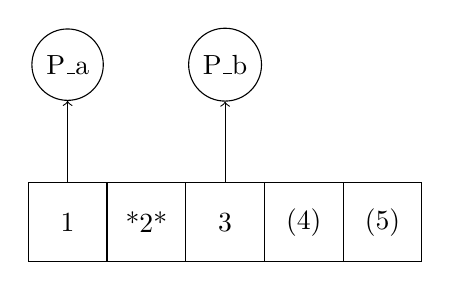
\begin{tikzpicture}
						\node[draw=black, text=black, shape=rectangle, minimum width=1cm, minimum height=1cm] (m_1) at (0,0) {1};
						\node[draw=black, text=black, shape=rectangle, minimum width=1cm, minimum height=1cm] (m_2) at (1,0) {*2*};
						\node[draw=black, text=black, shape=rectangle, minimum width=1cm, minimum height=1cm] (m_3) at (2,0) {3};
						\node[draw=black, text=black, shape=rectangle, minimum width=1cm, minimum height=1cm] (m_4) at (3,0) {(4)};
						\node[draw=black, text=black, shape=rectangle, minimum width=1cm, minimum height=1cm] (m_5) at (4,0) {(5)};

						\node[draw=black, text=black, shape=circle, minimum size=0.5cm] (p_a) at (0,2) {P\_a};
						\node[draw=black, text=black, shape=circle, minimum size=0.5cm] (p_b) at (2,2) {P\_b};

						\draw[->] (m_1.north) -- (p_a.south);
						\draw[->] (m_3.north) -- (p_b.south);
					\end{tikzpicture}
				\end{center}
				\caption{Le paragraphe A devient le noeud de départ}
			\end{figure}

			Dès lors, une case vide se retrouve disponible (symbolisé par des **). Ainsi, si l'on souhaite ajouter un noeud, il faudra d'abord combler ce vide. Le prochain paragraphe, le C donc, aura pour numéro le 2.

			\begin{figure}[H]
				\begin{center}
					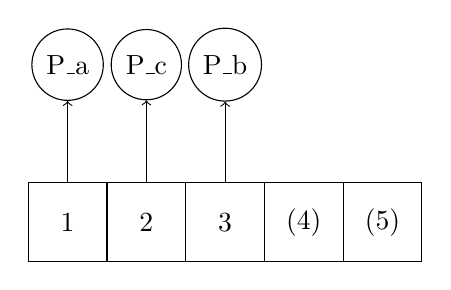
\begin{tikzpicture}
						\node[draw=black, text=black, shape=rectangle, minimum width=1cm, minimum height=1cm] (m_1) at (0,0) {1};
						\node[draw=black, text=black, shape=rectangle, minimum width=1cm, minimum height=1cm] (m_2) at (1,0) {2};
						\node[draw=black, text=black, shape=rectangle, minimum width=1cm, minimum height=1cm] (m_3) at (2,0) {3};
						\node[draw=black, text=black, shape=rectangle, minimum width=1cm, minimum height=1cm] (m_4) at (3,0) {(4)};
						\node[draw=black, text=black, shape=rectangle, minimum width=1cm, minimum height=1cm] (m_5) at (4,0) {(5)};

						\node[draw=black, text=black, shape=circle, minimum size=0.5cm] (p_a) at (0,2) {P\_a};
						\node[draw=black, text=black, shape=circle, minimum size=0.5cm] (p_b) at (2,2) {P\_b};
						\node[draw=black, text=black, shape=circle, minimum size=0.5cm] (p_c) at (1,2) {P\_c};

						\draw[->] (m_1.north) -- (p_a.south);
						\draw[->] (m_2.north) -- (p_c.south);
						\draw[->] (m_3.north) -- (p_b.south);
					\end{tikzpicture}
				\end{center}
				\caption{Ajout du paragraphe C}
			\end{figure}

			Enfin, notre application peut recommencer à ajouter des noeuds à la "fin" de notre Map.

			\begin{figure}[H]
				\begin{center}
					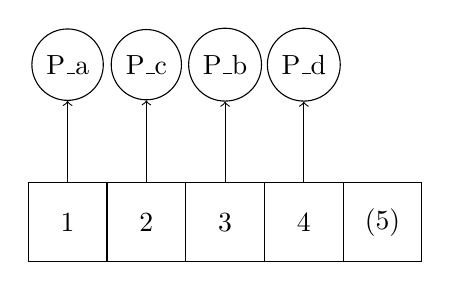
\begin{tikzpicture}
						\node[draw=black, text=black, shape=rectangle, minimum width=1cm, minimum height=1cm] (m_1) at (0,0) {1};
						\node[draw=black, text=black, shape=rectangle, minimum width=1cm, minimum height=1cm] (m_2) at (1,0) {2};
						\node[draw=black, text=black, shape=rectangle, minimum width=1cm, minimum height=1cm] (m_3) at (2,0) {3};
						\node[draw=black, text=black, shape=rectangle, minimum width=1cm, minimum height=1cm] (m_4) at (3,0) {4};
						\node[draw=black, text=black, shape=rectangle, minimum width=1cm, minimum height=1cm] (m_5) at (4,0) {(5)};

						\node[draw=black, text=black, shape=circle, minimum size=0.5cm] (p_a) at (0,2) {P\_a};
						\node[draw=black, text=black, shape=circle, minimum size=0.5cm] (p_b) at (2,2) {P\_b};
						\node[draw=black, text=black, shape=circle, minimum size=0.5cm] (p_c) at (1,2) {P\_c};
						\node[draw=black, text=black, shape=circle, minimum size=0.5cm] (p_d) at (3,2) {P\_d};

						\draw[->] (m_1.north) -- (p_a.south);
						\draw[->] (m_2.north) -- (p_c.south);
						\draw[->] (m_3.north) -- (p_b.south);
						\draw[->] (m_4.north) -- (p_d.south);
					\end{tikzpicture}
				\end{center}
				\caption{Ajout du paragraphe D}
			\end{figure}

			Voici quelques précisions supplémentaires :

			\begin{itemize}
				\item{Le principe d'indice manquant est le même pour la suppression d'un noeud}
				\item{Afin de gagner en performance pour déterminer le numéro d'un noeud déjà présent (pour savoir quel numéro sera manquant par exemple), une autre HashMap est mis à jour en même temps que celle des noeuds. Il s'agit de nodeInv. Cette map n'est rien de plus qu'une sorte de mirroir pour celle des noeuds, on lui passe un noeud en clé et on obtient son numéro. Il est donc extrêmement important que les deux maps soient parfaitement identique pour éviter tout bug.}
				\item{\label{subsec:noeud_delete_missing_index}Pour déterminer l'indice d'un noeud que l'on ajoute, nous nous basons sur la taille de la Map. Cela pose problème dans un cas particulié. En effet, si nous supprimons un paragraphe au milieu de la map, le noeud à l'indice 3 par exemple, alors cet indice sera libre. Si nous sauvegardons et décidons d'ouvrir de nouveau le fichier, alors nous n'aurons plus cette liste. Il faudrait que nous parcourions la Map pour trouver les indices manquant à la lecture du livre, cependant, comme évoqué un peu partout dans ce rapport, nous avons manqué de temps, d'autant plus que nous avons pensé à ce détails quelques jours avant de rendre le rapport.}
			\end{itemize}

			De ce fait, voici l'algorithme que nous avons mis en place pour l'ajout d'un noeud.

			\begin{algorithm}[H]
				\DontPrintSemicolon
				\KwIn{le noeud à ajouter : node}
				\KwData{
					nodes : Map<Integer, AbstractBookNode> liste des noeuds\;
					nodesInv : Map<AbstractBookNode, Integer> liste inversée des noeuds\;
					missingIndexes : List<Integer> liste des indices libres\;
				}

				\uIf{node in nodes}{
					\Return{}
				}

				\uIf{missingIndexes.length == 0}{
					offset: int\;
					offset $\gets$ (1 in nodes) ? 1 : 2\;
					nodes[nodes.length + offset] $\gets$ node\;
					nodesInv[node] $\gets$ nodesInv.length + offset\;
				}
				\uElse{
					nodes[missingIndexes[0]] $\gets$ node\;
					nodesInv[node] $\gets$ missingIndexes[0]\;
					missingIndexes.remove(0)\;
				}

				notifyNodeAdded(node)
				\caption{Ajout d'un noeud}
			\end{algorithm}

			La variable offset correspond au décalage à ajouter pour placer le noeud. Comme on commence à 2 un décalage de 2 est nécessaire. Supposons que le premier noeud est renseigné et qu'il est le seul du tableau, ajouter un nouveau noeud le placerait donc celui-ci à la position 2 + tailleDuTableau soit 2 + 1 c'est à dire 3. On a alors un décalage d'une "case". De ce fait, on doit faire un décalage de 1 uniquement si le premier noeud est renseigné.

			Voyons maintenant celui mis en place pour le changement du premier noeud.

			\begin{algorithm}[H]
				\DontPrintSemicolon
				\KwIn{le nouveau premier noeud : node}
				\KwData{
					nodes : Map<Integer, AbstractBookNode> liste des noeuds\;
					nodesInv : Map<AbstractBookNode, Integer> liste inversée des noeuds\;
					missingIndexes : List<Integer> liste des indices libres\;
				}

				\uIf{not (node in nodes)}{
					addNode(node)
				}
				\;
				updateDestinations(1, -1)\;
				\;
				indexOfNode: int\;
				indexOfNode $\gets$ nodesInv[node]\;
				\;
				oldNode: AbstractBookNode\;
				oldNode $\gets$ nodes[1]\;
				\;
				updateDestinations(indexOfNode, 1)\;
				\;
				nodes[1] $\gets$ node\;
				nodesInv[node] $\gets$ 1\;
				\;
				\uIf{oldNode != null}{
					nodes[indexOfNode] $\gets$ oldNode\;
					nodesInv[oldNode] $\gets$ indexOfNode\;

					updateDestinations(-1, indexOfNode)\;
				}
				\uElse {
					missingIndexes.add(indexOfNode)\;
					nodes.remove(indexOfNode)\;
				}

				\caption{Changement du premier noeud}
			\end{algorithm}

			\textit{NB: updateDestinations permet de changer les numéro de destination des BookNodeLink d'un ancien numéro, vers un nouveau}

			Si le noeud n'est pas présent dans le livre, nous commençons par l'ajouter. Les numéros des paragraphes vont êtres amenés à changer, de ce fait, il est important de mettre à jour les numéros de destination des différents liens. Nous commençons par déplacer les références du noeud 1 vers -1. En effet, cet indice n'est jamais renseigné. Ensuite, nous changeons les destination des liens qui allaient vers le "noeud à placer en premier" pour qu'elles pointent vers le premier noeud. Nous ajoutons le noeud à cette premiere "case". Deux options sont maintenant possibles. Il y avait déjà un premier noeud auparavant auquel cas il faut maintenant le placer là où se trouvait l'ancien et donc, mettre à jour les liens qui vont de -1 vers ce nouvel emplacement. Si jamais il n'y avait pas de premier noeud, alors une place est maintenant manquante. On l'ajoute donc à la liste des emplacements à combler avant de pouvoir de nouveau ajouter des noeuds normalement.

		\subsection{Le pattern observer et la classe Book}
			\label{subsec:pattern_observer}

			Le pattern observer est essentiel pour la mise en place du pattern MVC. Nous avons décidé de procéder de la manière suivante :

			\begin{figure}[H]
				\centering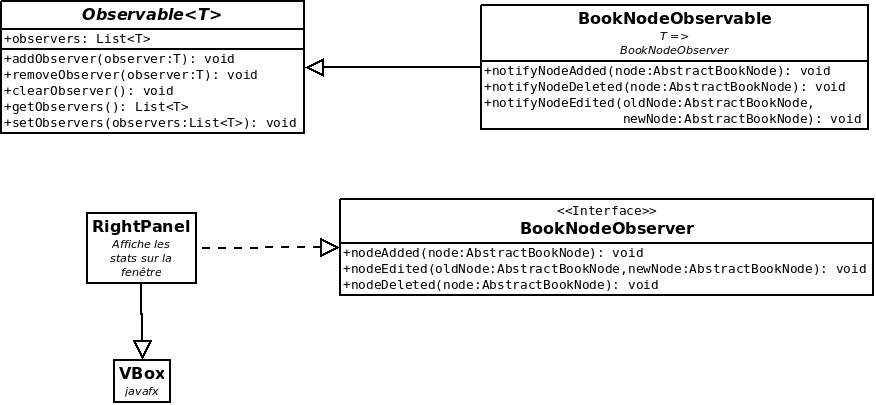
\includegraphics[width=0.8\textwidth, keepaspectratio]{img/observer.png}
				\caption{UML d'exmple sur le pattern observer}
			\end{figure}

			Comme on peut le voir, une classe mère \textbf{Observable<T>} détient une List<T> d'observers. Une méthode d'ajout, et de suppression permettent de modifier cette liste. Dès lors que l'on souhaite ajouter un nouveau type d'observer, on doit commencer par créer une nouvelle Interface avec les méthodes que l'on souhaite fournir, dans notre exemple il s'agit de nodeAdded, nodeEdited, nodeDeleted. Une fois cette interface faite, on doit alors faire une nouvelle classe Observable, BookNodeObservable dans notre cas, qui hérite de Observable<T>, T étant l'observer que l'on souhaite utiliser, donc BookNodeObserver. Ainsi, chaque Observable que l'on fera ne sera qu'une définition des méthodes pour notifier qu'un évènement s'est produit.

			Le choix à été fait de séparer les différentes parties (noeuds, liens, items, ...) du livre en différents observers afin de ne pas surcharger le nombre de méthodes à redéfinir dans les classes Observer, et donc de n'observer que ce dont on a besoin. De ce fait, tous les observers concernant le livre sont sont disponibles sauf celui pour notifier d'un changement concernant le premier noeud.

	\section{Lecture et écriture d'un livre}\label{sec:Json}

		L'objectif de l'application étant de concevoir un éditeur, il était important de permettre la sauvegarde et la lecture du livre que l'on édite. Le choix du format JSON est rapidement survenue. Premièrement car un fichier d'exemple qui nous a été fournis était sous ce format mais aussi car il s'agit d'une structure simple et très facile à lire. Nous avons alors utilisé GSON, une librairie, conçue par Google, extrêmement simple. Elle permet de retranscrire sous forme d'objet Java un fichier JSON structuré, c'est à dire où l'on distingue très clairement des objets qui se répète.

		Afin de lire un fichier JSON, avec cette librairie, il suffit de concevoir des objets Java avec les même attributs que ceux du fichier à lire ou à écrire. Voici un exemple très court de ce à quoi nos fichiers ressembles :

		\subsection{La structure du JSON}

			\begin{lstlisting}[gobble=12, language=json, caption=Exemple de livre très simple, label=lst:exemple_livre]
			{
				"prelude": "Vous êtes l'enseignant qui note notre projet",
				"setup": {
					"skills": [],
					"items": [],
					"characters": [],
					"character_creation": []
				},
				"sections": {
					"1" : {
						"text": "Vous être en train d'étudier notre projet",
						"choices": [
							{
								"text": "Mettre une bonne note",
								"section": 3
							},
							{
								"text": "Mettre une mauvaise note",
								"section": 2
							}
						]
					},
					"2": {
						"text": "Les étudiants du projet sont tristes",
						"end_type": "FAILURE"
					},
					"3": {
						"text": "Les étudiants sont satisfait de leur travail",
						"end_type": "VICTORY"
					}
				}
			}
			\end{lstlisting}

		On retrouve plusieurs éléments différents. On remarque par exemple un attribut "prelude", ainsi que deux grosses parties, "setup" et "sections". Dans la suite, nous détaillerons uniquement les attributs les plus frequemment présents.

		\subsubsection{Setup}

			Commençons par détailler "setup". Ce passage contient toutes les informations générales à notre livre. On y retrouve la liste des compétences ("skills"), la liste des items ("items") et la liste des personnages ("characters"). "character\_creation", lui, détaille toutes les étapes lors de la conception du personnage qui intervient au tout début. Celle-ci permet de sélectionner des skills et items de départ.

			Pour le moment les compétences sont uniquement composé d'un ID et d'un nom. Dans une future \maj{} il serait intéressant d'ajouter des propriétés pour connaitre la force ajouté dans un combat, la quantité de soins à rendre par noeuds, par exemple.

			\begin{lstlisting}[gobble=12, language=json, caption=Exemple de compétence]
			{
				"id": "sixth_sense",
				"name": "Sixième sens"
			}
			\end{lstlisting}

			Les items peuvent être de différents types : KEY\_ITEM, WEAPON, DEFENSE, MONEY, HEALING. On retrouve pour tous les items un id et un nom ("name"). Pour certains types, des attributs supplémentaires sont présent. Par exemple, un attribut "durability" peut être présent. Il permet de déterminer le nombre d'utilisation maximum d'un item. Un item de type HEALING possède un nombre de pv à rendre ("hp") tandis que ceux type WEAPON possède un montant de dégats ("damage") par exemple.

			\begin{lstlisting}[gobble=12, language=json, caption=Exemple d'items]
			{
				"id": "backpack",
				"name": "Backpack",
				"item_type": "KEY_ITEM"
			},
			{
				"id": "healing_potion_4",
				"name": "Potion de soins (4HP)",
				"hp": 4,
				"durability": 1,
				"item_type": "HEALING"
			}
			\end{lstlisting}

			Concernant les personnages on y retrouve un id, un nom ("name"), un nombre de pv maximum ("hp"), un boolean pour indiquer s'il a beaucoup de chance que ses coups fassent le double des dégats ("double\_damage"), ainsi que "combat\_skill" qui représente le montant de ses dégats.

			\begin{lstlisting}[gobble=12, language=json, caption=Exemple de personnage]
			{
				"id": "zombie_captain",
				"name": "Zombie Captain",
				"hp": 15,
				"double_damage": true,
				"combat_skill": 2
			}
			\end{lstlisting}

			Les character character\_creation peuvent être de simple texte ou de type "ITEM" ou "SKILL". On y retrouve les différents skills ou items que l'on peut prendre pour débuter notre aventure ainsi que le nombre maximum que l'on peut choisir ("amount\_to\_pick").

			\begin{lstlisting}[gobble=12, language=json, caption=Exemple de character\_creation]
			{
				"text": "Kai Disciplines\n\nOver the centuries, the Kai monks have mastered the skills of the warrior. These skills are known as the Kai Disciplines, [...]",
				"type": "SKILL",
				"skills": [
					"camouflage",
					"hunting",
					"sixth_sense",
					"tracking",
					"healing",
					"weaponskill",
					"mindshield",
					"mindblast",
					"animal_kinship",
					"mind_over_matter"
				],
				"amount_to_pick": 5
			}
			\end{lstlisting}

		\subsubsection{Sections}

			La partie "sections" est une map qui représente le numéro d'un paragraphe ainsi que le paragraphe associé. Il existe différents types de paragraphes : à choix, à choix aléatoire, avec des combats et terminaux. Tous possède un texte. Les noeuds terminaux possèdent un type de fin ("end\_type") afin savoir si l'on a gagné ou pas (cf : Listing \ref{lst:exemple_livre}). Les noeuds aléatoires eux, possèdent un attribut "is\_random\_pick" qui vaut true. Pour tous les autres types de noeuds, on retrouve parmis les attributs les plus importants une liste d'items qu'il est possible de prendre, un montant d'item maximum qui peut être pris ("amount\_to\_pick") et enfin des items disponibles à l'achat ("shop").

			\begin{lstlisting}[gobble=12, language=json, caption=Exemple de paragraphe]
			{
				"text": "The back door opens [...]",
				"items": [
					{
						"id": "gold",
						"amount": 5
					},
					{
						"id": "dagger"
					},
					{
						"id": "seal_hammerdal"
					}
				],
				"amount_to_pick": 2
				"choices": [
					{
						"text": "Return to the tavern.",
						"section": "177"
					},
					{
						"text": "Study the tomb.",
						"section": "24"
					}
				]
			}
			\end{lstlisting}

			Certains paragraphes peuvent contenir un attribut "combat". Dès lors on peut connaitre le choix en cas de victoire ("win"), de défaite ("loose") ou d'évasion ("evasion). Si l'évasion est possible seulement à partir d'un certains nombre de tour on retrouve alors un attribut nommé "evasion\_round". Pour finir, un attribut "enemies" permet de connaitre les personnages que l'on combat.

			\begin{lstlisting}[gobble=12, language=json, caption=Exemple de paragraphe avec des combats]
			{
				"text": "The dead zombies lie [...]",
				"combat": {
					"win": {
						"text": "If you win the combat.",
						"section": "309"
					},
					"enemies": [
						"zombie_captain"
					]
				}
			}
			\end{lstlisting}

			Pour représenter un lien vers un autre paragraphe on retrouve une liste de choix ("choices"). Ils possèdent également un texte qui correspond à l'intitulé du choix, le numéro du paragraphe suivant ("section"), un nombre d'hp à retirer, un nombre d'argent à ajouter ainsi qu'un liste de prérequis ("requirements"). Comme pour les BookNodeLink, il s'agit d'un tableau à deux dimensions. Le premier représente une liste de condition en OU et le second une liste de condition en ET. Enfin, pour les noeuds aléatoires, un probabilité est également présent ("weight").

			\begin{lstlisting}[gobble=12, language=json, caption=Exemple de choix]
			{
				"text": "If you have the Kai Discipline of Tracking.",
				"section": "182",
				"hp": -5,
				"requirements":  [
					[
						{
							"id": "tracking",
							"type": "SKILL"
						}
					]
				]
			}
			\end{lstlisting}

		\subsection{La lecture et l'écriture}
			\label{subsec:lecture_ecriture_fichier}

			Du fait que la structure en Json n'est pas identique à celle détaillé dans \nameref{sec:representation_livre} (page \pageref{sec:representation_livre}), nous avons fait des classes intermédiaires pour permettre cette lecture. Celles-ci sont disponibles dans le package \textit{magic\_book/core/file/json} et ne contiennent rien de plus que des getter et setter. Aussi, afin de permettre une convertion entre les classes faites pour représenter un fichier json et celles faites pour être utilisées par l'application, une interface \textit{JsonExportable} existe. Celle ci permet de redéfinir 2 méthodes. L'une renvoyant la classe JSON associé à notre classe actuelle, l'autre permettant à partir d'une classe JSON d'obtenir la classe Java correspondante.

			\begin{figure}[H]
				\centering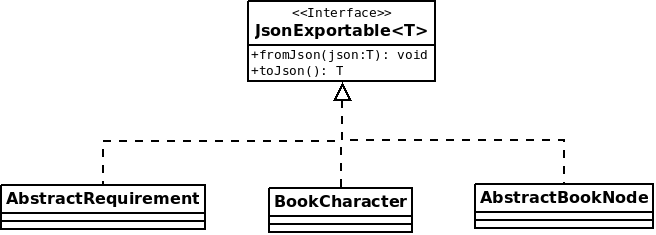
\includegraphics[width=0.66\textwidth, keepaspectratio]{img/json_exportable.png}
				\caption{L'interface JsonExportable et quelques classes qui l'implémentent}
			\end{figure}

			Enfin, les classes BookReader et BookWritter permettent de récupérer toutes les classes JSON intermédiaires pour les regrouper dans le BookJson qui correspond à la structure complète de notre livre. Ces classes sont également une couche d'abstraction à GSON car c'est elles qui se chargent d'écrire le JSON correspondant dans un flux.

			Pour résumer, on peut schématiser ces échanges de telle sorte :

			\begin{figure}[H]
				\begin{center}
					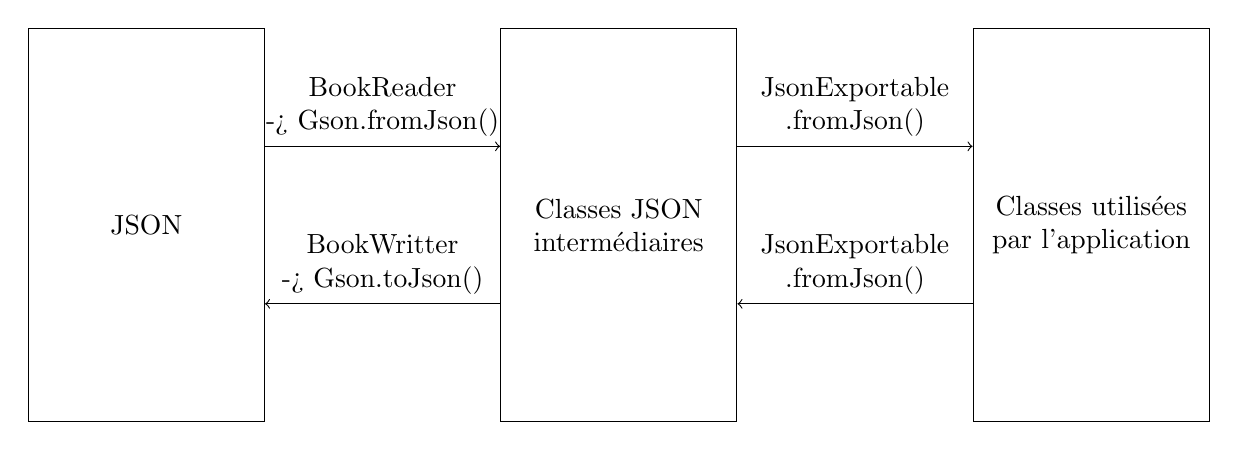
\begin{tikzpicture}
						\node[draw=black, text=black, shape=rectangle, minimum width=3cm, minimum height=5cm] (json) at (0,0) {JSON};
						\node[draw=black, text=black, shape=rectangle, minimum width=3cm, minimum height=5cm, align=center] (json_class) at (6,0) {Classes JSON\\ intermédiaires};
						\node[draw=black, text=black, shape=rectangle, minimum width=3cm, minimum height=5cm, align=center] (class) at (12,0) {Classes utilisées\\ par l'application};

						\draw[->] ([yshift=1cm]json.east) -- node[above, align=center] {BookReader\\ \fontsize{10}{12}\selectfont-> Gson.fromJson()}([yshift=1cm]json_class.west);
						\draw[->] ([yshift=-1cm]json_class.west) -- node[above, align=center] {BookWritter\\ \fontsize{10}{12}\selectfont-> Gson.toJson()}([yshift=-1cm]json.east);

						\draw[->] ([yshift=1cm]json_class.east) -- node[above, align=center] {JsonExportable\\.fromJson()}([yshift=1cm]class.west);
						\draw[->] ([yshift=-1cm]class.west) -- node[above, align=center] {JsonExportable\\.fromJson()}([yshift=-1cm]json_class.east);
					\end{tikzpicture}
				\end{center}
				\caption{Échanges pour la lecture / écriture}
			\end{figure}

	\section{Edition graphique d'un livre}

		\subsection{MainWindow}
			La MainWindow est notre fenêtre principale. Elle contient un Menu permettant de réaliser plusieurs actions ainsi que trois zones différentes (panel). Le premier panel se nomme le \textbf{LeftPane}. Il se situe à gauche et est composé de différent boutons permettant de changer de mode, de la liste des items et de personnage du livre. Le deuxième panel s'appel le \textbf{GraphPane}. Il est au centre et permet d'ajouter les noeuds ainsi que les liens entre les noeuds, c'est donc la zone d'édition de notre livre. Il contient également le prélude. Le troisième panel se nomme le \textbf{RightPane}. Il permet d'afficher les statistiques du livre comme par exemple, le nombre de noeud ainsi que l'estimation de la difficulté du livre.

			\begin{figure}[H]
				\centering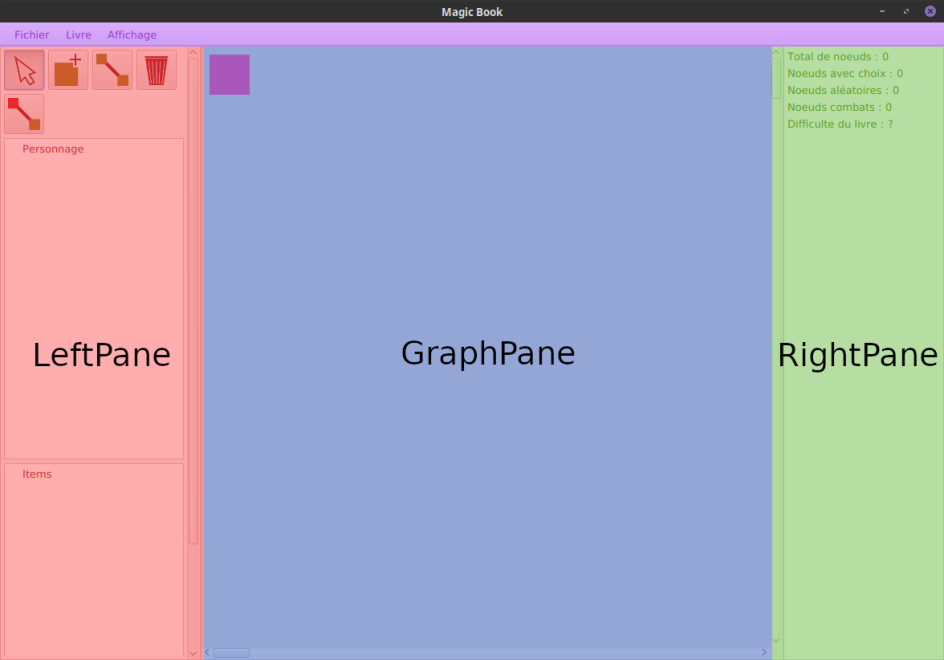
\includegraphics[width=0.50\textwidth]{img/mainwindow.png}
				\caption{MainWindow}
				\label{fig:MainWindow}
			\end{figure}

			Tout d'abord, dans la barre de menu de la fenêtre (menuBar), se trouve plusieurs onglets.
			Premièrement, dans le menu nommé \textbf{Fichier}, l'utilisateur peut alors ouvrir un nouveau livre vide en cliquant sur \textbf{Nouveau}. Le nouveau livre s'ouvre alors en mettant à jour tous les panels (LeftPane, GraphPane, RightPane), permettant ainsi de partir sur un nouveau livre. Ce menu comporte aussi un MenuItem nommé \textbf{Ouvrir}, permettant ainsi d'ouvrir un fichier Json ou txt. Si dans ce fichier, il manque une virgule ou une accolade ou autre ne permettant pas la lecture du fichier en Json (Voir \nameref{sec:Json} à la page \pageref{sec:Json}), un message d'erreur apparait. Si le fichier n'est pas bien fait, ne permettant pas l'ouverture de ce fichier, une classe nommée \textbf{BookValidator} devait "valider" le livre. Par manque de temps, cette classe n'est pas fonctionnelle. Si le fichier est correcte, le livre est chargé en mettant tous les panels à jour. Il peut aussi enregistrer ou enregistrer-sous le livre en faisant appel au FileChooser et au File.\\
			Deuxièmement, dans le menu nommé \textbf{Livre}, l'utilisateur peut \textbf{Jouer} ou \textbf{Estimer la difficulté}. Ces deux MenuItem utilisent tous les deux la classe Jeu, décrit un peu plus loin \nameref{sec:Jeu} à la page \pageref{sec:Jeu}. Un autre MenuItem est aussi présent, permettant de \textbf{Générer le livre en txt}. Cela permet à l'utilisateur de pouvoir avoir un livre propre au format texte.\\
			Troisièmement, dans le menu nommé \textbf{Affichage}, l'utilisateur peut afficher ou non, le LeftPane et/ou le RightPane. Cela permet notament à l'utilisateur de mieux voir la partie édition. Mais était surtout réalisé pour un meilleur affichage en vidéo projecteur de notre projet.


		\subsection{LeftPane}
			Ce panel contient tout d'abord des ToggleButton permettant de sélectionner un mode parmis cinq modes : \textbf{SELECT, ADD NODE, ADD NODE LINK, DELETE, FIRST NODE}. Ces modes sont sélectionnables à l'aide de bouton créé a partir de la méthode createToggleButton(). Cette méthode prend en paramètre une image et un des modes de la classe Mode. Un évènement est associé à chaque boutons permettant de changer le mode. Chaque mode permet d'executer des actions différentes, présenté ci-dessous. Les mêmes évènements de sélection, ainsi que de suppression, sont associés au lien.

			\begin{lstlisting}[gobble=12, language=java, caption=Modification Mode]
			class NodeFxListener implements RectangleFxObserver {
				@Override
				public void onRectangleFXClicked(RectangleFx rectangleFx, MouseEvent event) {
					NodeFx nodeFx = (NodeFx) rectangleFx;
					if(mode == Mode.SELECT){
						//sauvegarde du premier noeud cliqué
						if(event.getClickCount() == 2) {
							//Ouverture d'un NodeDialog
						}
					} else if(mode == Mode.ADD_NODE_LINK) {
						if(selectedNodeFx == null && !(nodeFx.getNode() instanceof AbstractBookNodeWithChoices)) {
							return;
						} else if(selectedNodeFx == null && nodeFx.getNode() instanceof AbstractBookNodeWithChoices) {
							//sauvegarde du premier noeud cliqué
						} else {
							//Création d'un lien entre les différents type du premier noeud
						}

					} else if(mode == Mode.DELETE) {
						//Supprime le noeud
					} else if(mode == Mode.FIRST_NODE) {
						//Modifie la destination du prélude
					}
					event.consume();
				}
			}
			\end{lstlisting}


			Une VBox est ensuite créé afin de mettre deux TreeView contenant un TreeItem pour la liste des items et un autre TreeItem pour celle des personnages. Il est possible d'ajouter des items et des personnages à partir de MenuItem (Ajout, Modification, Suppression) qui sont contenu dans un ContextMenu. Des évenèments sont liés à ces MenuItem afin de modifier le livre permettant d'appeler des méthodes afin de modifier la liste des items ou la liste des personnages.

			Prenons l'exemple d'un ajout d'un item. Un clique droit est alors enregistrer en tant qu'évènement. Ce clique permet de faire appel à la méthode handle() afin de créer un \textbf{ItemDialog} (boite de dialogue). La boite de dialogue est donc affiché, les valeurs peuvent être rentré. Si la boite n'est pas validé, aucun changement n'est effectué. Mais si l'utilisateur valide la boite, un \textbf{BookItem} est créé en fonction du type d'item (arme, un item de soin, de défense ou un simple item). L'item est alors ajouter dans le livre à l'aide d'une méthode addItem(). Cette méthode est présente dans la classe \textbf{Book}, permettant d'ajouter l'item et, dès ce faisant, notifier la classe \textbf{BookItemObservable} qu'un item a été ajouté. La méthode itemAdded() du \textbf{LeftPane} est alors appelé afin d'ajouter au treeView une vue sur l'item créer. Vous trouverez ci-dessous, la méthode si la captation d'un évènement "Ajouter un item" est enregistré. L'ajout d'un personnage se fait exactement dans la même idée.

			\begin{lstlisting}[gobble=12, language=java, caption=Ajout d'item]
			menuItemAdd.setOnAction(new EventHandler<ActionEvent>() {
				@Override
				public void handle(ActionEvent event) {
					ItemDialog itemDialog = new ItemDialog(LeftPane.this.book);
					BookItem item = itemDialog.getItem();
					if(item != null) {
						book.addItem(item);
					}
				}
			});
			\end{lstlisting}

			Prenons maintenant l'exemple d'une modification d'un item. Le même principe est effectué, sauf que l'item où il a été enregistré le clique, est envoyé dans la classe \textbf{ItemDialog}. L'item est alors modifié en fonction de son instanceof. Puis est modifié si le bouton "Valider" a été appuyé. La méthode updateItem est alors appelé de la classe \textbf{Book}. L'observeur fait maintenant appel à itemEdited(). Cette méthode permet de changer la valeur de l'item à l'aide d'un setValue. Vous trouverez ci-dessous, un exemple d'une modification d'un item.

			\begin{lstlisting}[gobble=12, language=java, caption=Modification d'item]
			menuItemUpdate.setOnAction(new EventHandler<ActionEvent>() {
				@Override
				public void handle(ActionEvent event) {
					TreeItem<BookItem> selectedItem = treeViewItem.getSelectionModel().getSelectedItem();
					if(selectedItem != null) {
						BookItem oldItem = selectedItem.getValue();

						ItemDialog newItemDialog = new ItemDialog(oldItem, LeftPane.this.book);
						BookItem newItem = newItemDialog.getItem();

						if(newItem == null){
							return;
						}

						book.updateItem(oldItem, newItem);
					}
				}
			});
			\end{lstlisting}

			Maintenant, prenons l'exemple d'une suppression d'item. Un enregistrement d'évènement est alors effectué sur "Supprimer un item". Une notification est envoyé directement dans le book, supprimant ainsi l'item et appelant la méthode du \textbf{LeftPane}, \textit{itemDeleted}. Cette méthode enlève alors du TreeView l'item supprimé à l'aide d'un remove(). Vous trouverez ci-dessous, le code de suppresion lors de l'enregistrement de l'évènement.

			\begin{lstlisting}[gobble=12, language=java, caption=Supression d'un item]
			menuPersoDel.setOnAction(new EventHandler<ActionEvent>() {
				@Override
				public void handle(ActionEvent event) {
					TreeItem<BookCharacter> selectedItem = treeViewPerso.getSelectionModel().getSelectedItem();
					book.removeCharacter(selectedItem.getValue());
				}
			});
			\end{lstlisting}


		\subsection{GraphPane}

			Le prélude est déjà situé en haut à gauche du GraphPane. Ce prélude, comme les noeuds, est représenté par un carré. Il contient un PréludeFx faisant le lien entre le noeud du prélude et le Rectangle le contenant. Ce prélude contient trois Tab. La première Tab contient le texte du prélude. La deuxième contient la création du personnage. Et la troisième la création du personnage principal.\\
			La deuxième partie du TabPane contient un Accordion. Cette accordion est affiché grâce au bouton \textbf{Ajouter}. Il est composé d'un CharacterCreationComponent comprenant un Texte, une CheckBox (Texte, Item), et d'un bouton \textbf{Supprimer cette partie}.\\
			La checkBox n'affiche que \textbf{Texte} si aucun item n'est disponible. Mais si un item est créé, l'utilisateur peu alors ajouter un ItemListComponent en sélectionnant \textbf{Item} dans la CheckBox. Cette classe est affiché sur tout les noeuds, permettant d'ajouter des items ainsi que la quantité disponible de chaque item, qui ici, sera disponible en début de partie. L'item ajouté peut être supprimé grâce à un clic droit de la souris.\\
			La troisième partie du TabPane permet quant a elle, de créer le personnage principal grâce au CharacterComponent. Cette classe permet de créer un personnage. Mais si la valeur boolean de mainCharacter est true, les TextField pour le nombre d'item maximum ainsi que la quantité d'argent est ajouté.
			Après validation, le textPrelude (texte du prélude), mainCharacter (personnage principal) et le characterCreations (item et texte à afficher après le prélude) est créer.

			Maintenant que vous avez une vision du prélude, une présentation de son code s'impose. Tout d'abord, le prélude contient donc la classe \textbf{RectangleFx}. Cette classe envoie donc une notification si un évènement \textit{Mousse} est enregistré. Cette évènement est recu par le \textbf{PréludeFx}, qui lui, regarde si le mode \textbf{SELECT} est activé. Si ce mode est activé et deux cliques sont enregistré sur le prélude, ce dernier ouvre sa boite de dialog avec, ou non, des informations à l'intérieur (si c'est une modification).\\
			Dès que le prélude est valider, le book modifie son prélude, le personnage principal ainsi que le characterCreations (ajout des items, texte). Ci dessous, vous découvrirez le code de modification du prélude.

			\begin{lstlisting}[gobble=12, language=java, caption=Ajout / modification du prélude]
			private void createNodePrelude() {
				PreludeFx preludeFx = new PreludeFx(zoom);
				preludeFx.setRealX(10);
				preludeFx.setRealY(10);

				preludeFx.addNodeFxObserver((RectangleFx rectangleFx, MouseEvent event) -> {
					if(mode == Mode.SELECT) {
						if(event.getClickCount() == 2) {
							PreludeDialog dialog = new PreludeDialog(book);

							if(dialog.getTextePrelude() != null) {
								book.setTextPrelude(dialog.getTextePrelude());
								book.setMainCharacter(dialog.getMainCharacter());
								book.setCharacterCreations(dialog.getCharacterCreations());
							}
						}
					}
				});

				preludeFxFirstNodeLine.startXProperty().bind(preludeFx.xProperty().add(preludeFx.widthProperty().divide(2)));
				preludeFxFirstNodeLine.startYProperty().bind(preludeFx.yProperty().add(preludeFx.heightProperty().divide(2)));

				rootPane.getChildren().add(preludeFx);
				this.setPreludeFx(preludeFx);
			}
		\end{lstlisting}


			Concernant l'ajout d'un noeud, on clique sur le mode \textbf{ADD\_NODE},puis on clique sur le GraphPane. Une méthode \textit{createNodeFxDialog} est alors appelé.

			\begin{lstlisting}[gobble=12, language=java, caption=ADD NODE()]
				public NodeFx createNodeFxDialog(MouseEvent event){
					NodeDialog nodeDialog = new NodeDialog(book);
					AbstractBookNode node = nodeDialog.getNode();

					if(node != null) {
						lastXClick = event.getX();
						lastYClick = event.getY();

						book.addNode(node);
					}

					return null;
				}
			\end{lstlisting}

			Une fenêtre de dialog est alors ouverte afin de renseigner le paragraphe à afficher, ainsi qu'une CheckBox permettant de sélectionner le type de noeud. L'affichage change en fonction du type de noeud sélectionner dans cette CheckBox, qui elle, est prédéfini sur \textbf{Basic}.

			Si c'est un noeud basic ou aléatoire, les renseignements suivant sont demandé: le texte à afficher, le nombre de points de vie à gagner/perdre, les items disponible, le nombre d'item disponible. Rien ne change sur la structure de la boite de dialog entre ces deux types. Mais au moment de la validation, le type de BookNode créer se fera en fonction de la valeur de la choiceBox : BoockNodeWithChoices, BookNodeWithRandomChoices. Des try/catch sont utilisé afin de changer certaine valeurs de saisie en Integer. Cela permet d'être sûr que ce sont des chiffres. Si la conversion ne peut pas se faire, une boite de dialog affichant l'erreur apparait, notifiant ainsi où l'erreur se situe.

			Si c'est un noeud terminal, une ChoiceBox est juste rajouté afin de savoir si c'est un noeud gagnant ou perdant. Lors de la validation, un BookNodeTerminal est créer avec comme valeur un BookNodeStatus défini en fonction de la ChoiceBox.

			Dès qu'un noeud est validé, la méthode \textit{createNodeFxDialog} envoie une notification au \textbf{Book} permettant que le noeud créer soit ajouté dans la liste. Une fois cela effectué, un observeur est notifié afin d'effectuer un appel à la méthode \textit{nodeAdded} dans le \textbf{GraphPane}. Cette méthode permet de créer le \textbf{NodeFx} qui extend de \textbf{Rectangle Fx}.

			\begin{lstlisting}[gobble=12, language=java, caption=Création du NodeFxDialog]
			public NodeFx createNode(AbstractBookNode node, double x, double y) {
				NodeFx nodeFx = new NodeFx(node, zoom);
				nodeFx.setRealX(x/zoom.get());
				nodeFx.setRealY(y/zoom.get());

				nodeFx.addNodeFxObserver(new NodeFxListener());

				listeNoeud.add(nodeFx);
				rootPane.getChildren().add(nodeFx);

				lastXClick = 0;
				lastYClick = 0;

				return nodeFx;
			}
			\end{lstlisting}

			Il contient alors le noeud créer et affiche un Rectangle là où la souris a été cliqué dans le graphPane, à la création du noeud. La couleur du carré change en fonction du type de noeud. Un RectangleFX est donc mis en place permettant d'envoyé une notification si jamais la souris passe dessus (opacité du Rectangle qui change), réalise un clique maintenu (déplacement du rectangle en fonction de la souris), réalise un clique simple. Pour ce dernier, cela envoie une notification à l'observable permettant de prévenir l'observeur qu'on a cliquer dessus. Cela sert si un double clique est produit (permet de procédé à une modification si le mode activé est \textbf{SELECT}, a une suppression si c'est le mode \textbf{DELETE} qui est activé ou encore a une création de lien entre le prélude et le noeud sélectionné si le mode \textbf{FIRST\_NODE} est activé) ou si un deux cliques espacé sont réalisé (permet de procédé à la création d'un lien si le mode \textbf{ADD\_NODE\_LINK} est sélectionné).


			Une fois un ou plusieurs noeud créer, un lien peut être donc être effectué. Le lien peut être fait sur le même noeud, si une boucle est voulu. Mais il peut aussi être réalisé entre deux noeuds. Pour ce faire, le mode \textbf{ADD\_NODE\_LINK} doit être activé. Le premier clique permet de sauvegarder le noeud de départ. Le deuxième permet d'avoir le noeud de destination. Une fois les deux cliques détecté, une fenêtre de dialog apparait alors.

			Il y a trois affichage différent. L'affiche ce fait en fonction du premier noeud. Tout d'abord, l'affichage commun entre ces noeuds est un simple texte, deux TextField ainsi qu'un CheckBox. Les TextField permettent d'ajouter un gain ou une perte de vie/d'argent. La CheckBox, quant a elle, permet d'aller vers ce choix obligatoirement ou non.\\
			Si le premier noeud est un noeud de combat, une ChoiceBox apparait alors permettant de choisir si c'est un lien gagnant, perdant ou un lien d'évasion. Cette liste de choix est créer si le permier noeud à encore des choix de libre. S'il n'a plus de choix libre, une boite d'alerte s'affiche en prévenant qu'il n'y a plus aucun lien disponible.

			Si le permier noeud est de type aléatoire, le joueur doit alors renseigner la chance sur chaque lien.

			Une fois la boite de dialogue validé, une méthode est appelée dans la Classe \textbf{Book}, afin d'ajouter le lien ainsi que de notifier le \textbf{BookNodeLinkObservable}. Cet observeur va alors appeler la méthode \textit{nodeLinkAdded} permettant de créer une ligne entre le NodeFx de départ et le NodeFx de destination. Pour différencier les deux, un cercle est créé et est affiché au noeud de destination. Tout cela est géré par NodeLinkFx qui a aussi un observeur permettant d'envoyer une notification si jamais la ligne ou le cercle enregistre un événement du style "pressed". Cela permet de savoir si le lien a été double cliqué pour réaliser une modification.\\
			Ce NodeLinkFx est créer dans la méthode \textit{createNodeLink}, défini ci-dessous.

			\begin{lstlisting}[gobble=12, language=java, caption=Création du lien NodeLink]

			public NodeLinkFx createNodeLink(BookNodeLink bookNodeLink, NodeFx firstNodeFx, NodeFx secondNodeFx) {
				NodeLinkFx nodeLinkFx = new NodeLinkFx(bookNodeLink, firstNodeFx, secondNodeFx, zoom);
				nodeLinkFx.addNodeLinkFxObserver(new NodeLinkFxListener());

				nodeLinkFx.startXProperty().bind(firstNodeFx.xProperty().add(firstNodeFx.widthProperty().divide(2)));
				nodeLinkFx.startYProperty().bind(firstNodeFx.yProperty().add(firstNodeFx.heightProperty().divide(2)));

				nodeLinkFx.endXProperty().bind(secondNodeFx.xProperty().add(secondNodeFx.widthProperty().divide(2)));
				nodeLinkFx.endYProperty().bind(secondNodeFx.yProperty().add(secondNodeFx.heightProperty().divide(2)));

				listeNoeudLien.add(nodeLinkFx);

				nodeLinkFx.registerComponent(rootPane);

				return nodeLinkFx;
			}

			\end{lstlisting}

		\subsection{RightPane}

		Ce panel contient tout ce qui représente les statistiques. Dès qu'un noeud est ajouté ou supprimé, une méthode de la class \textit{RightPane} est utilisé afin de mettre à jour le nombre de noeuds existant. Pour la difficulté du livre, elle est mise à jours dès que \textbf{Estimé la difficulté du livre} est sélectionné.\\
		Si un nouveau livre est chargé, tout ces statistiques ce remmettent à zéro.



	\section{Rendre le livre jouable et estimer sa difficulté}\label{sec:Jeu}
		\subsection{Jeu}
		Une classe à été créer se nommant \textbf{Jeu}, permettant de gérer les méthodes de jeu communes entre le \textit{Player} et les \textit{Fourmis}.\\
		Un construteur est d'abord appelé, à partir de la MainWindow, afin d'envoyer le livre contenant toutes les informations. Puis, en fonction du mode sélectionner (\textbf{Générer la difficulté} ou \textbf{jouer}), la méthode correspondante au player est appelé.\\
		Une fois dans la méthode choisis, la méthode \textit{runGame()} est alors appelé. Le livre est copié, afin de ne pas le modifier par erreur pendant le jeu. Un BookState, qui correspond à l'état de la partie, est alors créé. Si le prélude contient un personnage principal, alors celui-ci est enregistré dans le BookState. Dans le cas contraire, un autre personnage principal est créé afin de pouvoir jouer au jeu (voir méthode si dessous).

		\begin{lstlisting}[language=java, caption=createNewState()]
			BookState newState = new BookState()
			if(this.book.getMainCharacter() == null){
				//Création d'un BookCharacter
			} else {
				BookCharacter bookCharacterMain = this.book.getMainCharacter();
			}
			newState.setBook(this.book);
			for(AbstractCharacterCreation characterCreation : this.book.getCharacterCreations())
				player.execPlayerCreation(book, characterCreation, newState);

			return newState;
		\end{lstlisting}

		Enfin, si des compétences et/ou des items sont disponible au début de la partie, la méthode de création de joueur (\textit{execPlayerCreation}, voir \ref{execPlayerCreationCode}) est appelé en fonction du player actuel. Comme cela, le player choisit parmi une liste de skill et d'items disponible en début de partie afin de les avoir pour commencer le jeu.\\
		Une fois le BookState créé, le personnage principal initialisé et la copie du livre enregistré, le premier noeud est donc chargé. La boucle while du runGame() est donc lancé et ne s'arrètera qu'une fois la partie terminé. Comme vous pouvez le remarquer, sur le code ci-dessous, chaque méthode correspond à un type de noeud en particulier. Les méthodes s'exécutent alors, puis renvoie le noeud de destination, en fonction du choix du player et / ou de la mort du player. Durant l'exécution des différentes méthodes et en fonction du player, d'autres méthodes externe sont appelées nottament dans la classe Fourmis ou Player.

		\begin{lstlisting}[language=java, caption=Méthode runGame()]
			while(!gameFinish){
				if(currentNode instanceof BookNodeCombat){
					//execNodeCombat(bookNodeCombat);
				}
				else if(currentNode instanceof BookNodeWithChoices){
					//execNodeWithChoices(bookNodeWithChoices);
				}
				else if(currentNode instanceof BookNodeWithRandomChoices){
					//execNodeWithRandomChoices(bookNodeWithRandomChoices);
				}
				else if(currentNode instanceof BookNodeTerminal){
					//execNodeTerminal(bookNodeTerminal);
					//Si partie gagné, win = true
				} else {
					//BookNodeTerminal FAILURE
				}
			}
			return win;
		\end{lstlisting}

		Pour chaque type de noeud, sauf pour un noeud terminal, une méthode commune est appelé afin de savoir si le noeud pris en charge fait gagné/perdre de la vie, puis regarde si le player est toujours en vie. Si ce dernier n'est plus en vie, un noeud terminal est alors renvoyé en noeud de destination. S'il est encore en vie et que le noeud propose des items, ils sont proposés au player en appelant la méthode correspondante entre Fourmis ou Player. A chaque detination choisi, une autre méthode est appelé afin de regarder si le lien entre le noeud de départ et de destination fait perdre ou gagner de la vie et/ou de l'argent.

		\textbf{Si un noeud est de type basic}, il est alors pris en charge dans la méthode \textit{execNodeWithChoices}. Cette dernière renvoi un noeud terminal si aucun choix n'est valide, ce qu'il veut dire, si le player n'a aucun choix ou s'il ne possède pas les items/skill pour aller vers ce choix.\\
		Si le player est encore en vie et si il peut au moins choisir une destination, un choix est demandé parmis toutes les destinations faisant un appel à la méthode en fonction du player. Si le player a les prérequis pour aller vers cette destination, alors le noeud choisi est renvoyé en noeud de destination. Sinon, le player doit faire un autre choix.


		\begin{figure}[H]
			\centering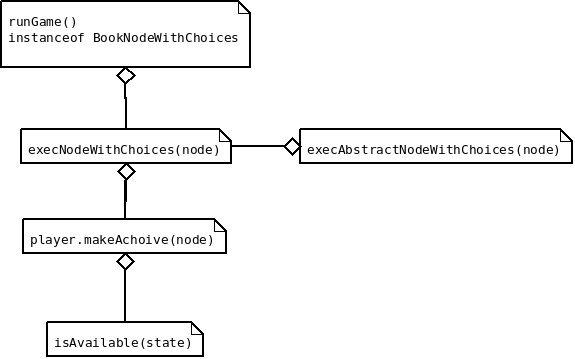
\includegraphics[width=0.70\textwidth]{img/JeuBookNodeWithChoices.png}
			\caption{Jeu BookNodeWithChoices}
			\label{fig:JeuBookNodeWithChoices}
		\end{figure}


		\textbf{Si c'est un noeud de type combat}, une vérification est réalisé afin savoir si le noeud contient des ennemis. S'il n'y a pas d'ennemis, le noeud en cas de victoire est envoyé en noeud de destination. Sinon, une liste d'ennemis est créer afin de ne pas modifié la vie des ennemis. Car ces derniers ne sont pas lié au noeud, mais c'est l'ID de l'ennemis qui est lié au noeud permettant de les appelés plusieurs fois dans plusieurs ou dans le même noeud.\\
		Le combat commence alors. Le choix est défini par la méthode du player correspondant. Trois choix sont possible:

		\begin{description}
			\item[Attaque :]{un autre choix (cf ligne 2) est demandé permettant de sélectionner l'ennemi à attaquer parmi la liste des ennemis encore en vie. Une fois l'ennemi sélectionné, une méthode attaque (cf ligne 7) est appelé apellant elle même une autre méthode commune entre l'attaque du player et l'attaque d'ennemi. Nommé \textit{getDamageAmount}, elle permet de savoir le nombre de dommage réalisé en fonction des point d'attaque de l'attaquant, de son double dommage décider en random si ce boolean est défini en true, d'un coup critique décider aussi en random, de l'arme de l'attaquant et de l'item de défense de l'attaqué. L'attaquant et l'attaqué est défini en fonction de la permière méthode qui l'appel. Ici c'est la méthode d'attaque du player.}
			Une fois l'attaque effectué, si l'ennemi attaqué est mort, il est supprimer de la liste des ennemis (cv logne 9)
			\item[Inventaire :]{si ce choix est fait par le player, la méthode appelé permettant d'utiliser son inventaire est elle même gérer dans la classe Player ou la classe Fourmis. Elle permet alors de choisir une potion, une arme et ou un item de défense.}
			\item[Evasion :]{si le tour avant évasion est inférieur ou égal à 0 (voir cf 13) et si un noeud de d'évasion existe, le player peut alors s'enfuir. Sinon cela lui passe son tour.}
		\end{description}

		\begin{lstlisting}[caption=JeuCombat]
		while(!finCombat){
			ChoixCombat choixCombat = player.combatChoice(node, evasionRound, state);

			if (choixCombat == ChoixCombat.ATTAQUER) {

				BookCharacter ennemi = player.chooseEnnemi(listEnnemis);
				attaque(ennemi);
				if(!ennemi.isAlive()){
					listEnnemis.remove(ennemi);
				}
			}
			else if(choixCombat == ChoixCombat.EVASION) {
				if(evasionRound <= 0 && node.getEvasionBookNodeLink() != null){
					execBookNodeLink(node.getEvasionBookNodeLink());
					return book.getNodes().get(node.getEvasionBookNodeLink().getDestination());
				}
			}

			ennemiTour(listEnnemis);

			if(!state.getMainCharacter().isAlive()) {
				//Vérification d'un noeud Failure
				if(node.getLooseBookNodeLink() != null)  {
					execBookNodeLink(node.getLooseBookNodeLink());
					return book.getNodes().get(node.getLooseBookNodeLink().getDestination());
				} else
					return new BookNodeTerminal("Vous succombez à vos blessures", BookNodeStatus.FAILURE);
			}

			if(listEnnemis.isEmpty())
				finCombat = true;

			evasionRound -= 1;
			}
		\end{lstlisting}

		Une fois le tour du joueur fini, vient le tour de l'ennemi. Il appel une méthode envoyant la liste d'ennemis restant. Cette méthode appel \textit{getDamageAmount} permettant aux ennemis d'attaquer un par un.

		La fin de combat est déterminé si la liste d'ennemis est vide ou si le player n'est plus en vie. Le noeud de destination est alors défini en fonction du résultat en fin de combat.

		\textbf{Si le noeud est de type aléatoire}, la méthode commune est appelé afin de savoir si le player est encore en vie. Puis une autre méthode, nommé getRandomChoices() ( voir \ref{getRandomChoices} à la page \pageref{getRandomChoices}) est appelé de la classe BookNodeLinkRandom afin de déterminer le noeud de destination en fonction des chances attribué à chacun de ces choix.

		\textbf{Si le noeud est de type terminal}, la partie est alors terminé et renvoie un bolean sur l'état de la fin de partie.

	\subsection{Interface Player / Foumis}
		Une interface \textbf{InterfacePlayerFoumis} à été créer permettant une mise en commun des codes Player et Fourmis. Ces méthodes permettent de faire un choix, prendre les items disponibles, créer un personage lambda, aller dans l'inventaire, choisir son ennemis ou encore combatre. Elles sont appelé au même moment. La méthode sera alors exécuté différément en fonction du player.

		\textit{execPlayerCreation} permet de choisir les skill et les items disponible au début de la partie. Ces derniers sont défini lors de la création du prélude. Pour l'ajout des items, la méthode \textit{prendItems} est appelé.

		\textit{combatChoice}, prend en paramètre le noeud de Combat et le nombre de tour avant l'évasion ainsi que le BookState, permet de faire un choix lors du tour du player dans un combat. On peut alors choisir d'attaquer, d'aller dans l'inventaire ou alors de s'évader. Si on choisi l'inventaire, on va alors dans une autre méthode appelé useInventaire() qui prend le BookState en paramètre. On peut alors utiliser une potion, prendre un objet de défense ou alors une arme. Si l'on choisis un autre choix, cette objet n'est pas utilisable lors d'un combat (comme par exemple de l'argent). Une fois l'objet pris, on retourne dans les choix du combat. On peut alors, soit retourner dans l'inventaire pour prendre un autre objet, soit attaquer ou s'évader.

		\textit{chooseEnnemi} permet de choisir l'ennemi à attaquer parmi la liste de tout les ennemis encore en vie.

		\textit{prendItems} permet de prendre un item parmi la liste d'items disponible. Cette liste est pris en paramètre ainsi que la sauvegarde de la partie et le nombre d'item maximum pouvant être pris.

		\textit{makeAChoice} permet de faire un choix en fonction des différentes destinations proposé par le noeud.

		\textit{useIventaire} permet d'utiliser son inventaire lors d'un noeud de combat. La mise à jour d'un port d'item de défense ou d'arme est alors mis à jour. Si un item de soin est choisi, les points de vie du joueur sont alors actualisé.

	\subsection{Player}
		La classe \textbf{Player} permet de jouer au jeu en tant que joueur. Elle permet de faire des choix grâce aux Scanner. Des messages sont aussi affiché afin de guider le joueur dans ses choix.\\
		Notament la méthode \textit{choixYesNo} qui permet de choisir oui ou non et de renvoyer le boolean true ou false. Cette méthode permet, par exemple, de savoir si le player veut supprimer, prendre un item ou un skill.\\
		Pour la méthode commune \textit{prendItems}, cette dernière fait appel à d'autre méthode dans la classe Player. Comme \textit{itemAdd} (cf ligne 15) permettant de choisir l'item à ajouter dans l'inventaire. Ou encore \textit{itemPlein} (cf ligne 8) qui demande au joueur s'il veut supprimer un item. Si le joueur répond oui (condition à ligne 10), la méthode \textit{itemSupp} (implémenté dans la méthode \textit{itemPlein}) est appelé afin de choisir l'item à supprimer et à mettre à jour l'inventaire grâce au state pris en charge dans la méthode0\textit{prendreItems}

		\begin{lstlisting}[gobble=12, language=java, label=prendreItems]
			public void prendreItems(BookState state, List<BookItemLink> bookItemLinks, int nbItemMax){
				while(nbItemMax != 0 && !bookItemLinks.isEmpty()){
					//affichage des choix
					//Voulez vous un item
					if(choixYesNo()){
						int itemMax = state.getMainCharacter().getItemsMax();
						if(itemMax == state.getMainCharacter().getItems().size()){
							itemPlein(state);
							//Choisir item:
							if(choixYesNo())
								nbItemMax = 0;
							else
								itemSupp(state);
						} else {
							itemAdd(state, bookItemLinks);
						}

					} else {
						nbItemMax = 0;
					}

					if(bookItemLinks.isEmpty())
						nbItemMax = 0;
				}
			}
				\end{lstlisting}

		Pour la méthode \textit{execPlayerCreation} au moment de l'ajout des skill, le joueur doit confimer ou non s'il veut un skill. Si oui, la méthode skillAdd est appelé jusqu'à ce que le maximum de skill à été pris ou qu'il n'en reste plus à prendre. Pour les items, la méthode \textit{prendItems}, défini ici\ref{prendreItems} est utilisé.

		\begin{lstlisting}[gobble=12, language=java, label=execPlayerCreationCode]
		public void execPlayerCreation(Book book, AbstractCharacterCreation characterCreation, BookState state){
				if(characterCreation instanceof CharacterCreationItem){
					CharacterCreationItem characterCreationItem = (CharacterCreationItem) characterCreation;
					prendreItems(state, characterCreationItem.getItemLinks(), characterCreationItem.getAmountToPick());
				}
				else if(characterCreation instanceof CharacterCreationSkill){
					CharacterCreationSkill characterCreationSkill = (CharacterCreationSkill) characterCreation;

					int nbItemMax = characterCreationSkill.getAmountToPick();

					while(nbItemMax != 0 && !characterCreationSkill.getSkillLinks().isEmpty()){
						int i = 0;
						skillAdd(state, characterCreationSkill);
						nbItemMax--;
					}
				}
			}
		\end{lstlisting}

	\subsection{Fourmis}
		La classe \textbf{Fourmis} permet de jouer en tant que joueur fictif. Elle effectue des choix random en fonction des différentes méthodes de l'interface.
		Comme par exemple, pour prendre des items ou des skill, la fourmi en prend autant que possible et en supprime obligatoirement en aléatoire si il n'a plus de place dans l'inventaire. Nous avons décider de réalisé cette méthode comme cela afin de pouvoir aller dans le maximum de noeud s'ilsont des prérequis ou alors avoir le maximum d'items pour les combats.\\
		Pour la méthode \textit{chooseEnnemi}, la fourmi envoyé prend obligatoirement le premier ennemi permettant de tué le maximum d'ennemis en attaquant toujours le même ennemis.\\
		Et enfin, la méthode \textit{combatChoice} permet de choisir entre ATTAQUE, EVASION, INVENTAIRE. Nous avons choisir de faire un random sur les trois choix et non pas sur deux choix même si le tour d'évasion n'est pas disponible afin de passer le tour, comme le joueur, afn d'avoir la même chance lors des combats.
